% Define some useful global switches...
\newif\ifDraft
\newif\ifNoFloat
%-------------------------------------------------------------------------------

% When "true", output in "draft" mode -- useful for proofing
\Draftfalse

% When "true", put listings, figures and tables where you put them, instead of floating:
\NoFloattrue
%-------------------------------------------------------------------------------

\newif\ifArticle  \Articlefalse
\newif\ifTwoColumn\TwoColumnfalse
%-------------------------------------------------------------------------------

\ifDraft
  \documentclass[onecolumn, a4paper, 12pt, titlepage, fleqn, oneside]{book}
\else
  \ifFormal
    \documentclass[onecolumn, a4paper, 11pt, titlepage, fleqn]{book}
  \else
    \documentclass[onecolumn, a4paper, 11pt, titlepage, fleqn, oneside]{book}
  \fi
\fi
\bibliographystyle{IEEEtran}
%-------------------------------------------------------------------------------

% Widen the text area
\usepackage{a4wide}

% Swap the margins around
\newlength{\TempLength}
\setlength{\TempLength}    {\oddsidemargin}
\setlength{\oddsidemargin} {\evensidemargin}
\setlength{\evensidemargin}{\TempLength}

% Use "blocky" paragraphs
\setlength{\parskip}{1em}
\setlength{\parindent}{0mm}
%-------------------------------------------------------------------------------

\ifFormal
  \usepackage{fancyhdr}
  \pagestyle{fancy}
  \fancyhead{}
  \fancyhead[LE]{\thepage}
  \fancyhead[RE]{\leftmark}
  \fancyhead[LO]{\rightmark}
  \fancyhead[RO]{\thepage}
  \setlength{\headheight}{15pt}
  
  \fancyfoot{}
  
  % Make empty pages before chapters truly empty (from fancyhdr manual)
  
  \makeatletter
   \def\cleardoublepage{\clearpage\if@twoside \ifodd\c@page\else
    \mbox{}
    \thispagestyle{empty}
    \newpage
    \if@twocolumn\hbox{}\newpage\fi\fi\fi}
  \makeatother
\else
  \pagestyle{plain}
\fi
%-------------------------------------------------------------------------------

\newcommand{\Chapter}[1]{%
 \chapter{#1}%
 \addcontentsline{lof}{chapter}{\thechapter{}~~#1}%
 \addcontentsline{lot}{chapter}{\thechapter{}~~#1}%
}

\makeatletter
  \renewcommand\subsubsection{\@startsection{subsubsection}{3}{\z@}%
                             {-3.25ex\@plus -1ex \@minus -.2ex}%
                             {1.5ex \@plus .2ex}%
                             {\refstepcounter{subsubsection}\normalfont\normalsize\bfseries\thesubsubsection~~~}}
\makeatother
%-------------------------------------------------------------------------------

%-------------------------------------------------------------------------------

\begin{document}
\begin{sloppypar}

\title{Large Template}


\begin{titlepage}
	\centering
	\vspace*{0.5 cm}
	
\includegraphics[scale = 0.5]{Figures/UCT.jpg}\\[1 cm]	% University Logo
	\textsc{\LARGE University of Cape Town}\\[2.0 cm]	% University Name
	\textsc{\Large SUBJECT CODE}\\[0.5 cm]				% Course Code
	\textsc{\large Subject Name}\\[0.5 cm]				% Course Name
	\rule{\linewidth}{0.2 mm} \\[0.4 cm]
	{ \huge \bfseries Title of Paper}\\
	\rule{\linewidth}{0.2 mm} \\[1.5 cm]
	
	\begin{minipage}{0.4\textwidth}
		\begin{flushleft} \large
			\emph{Authors:}\\
			Author 1\\
            Author N
		\end{flushleft}
	\end{minipage}~
	\begin{minipage}{0.4\textwidth}
		\begin{flushright} \large
			\emph{Student Numbers:} \\
			STUDNUM1\\	
            STUDNUMN
            % Your Student Number
		\end{flushright}
	\end{minipage}\\[2 cm]
	
	{\large 22 April 2018}\\[2 cm]
	
	\vfill
	
\end{titlepage}
\title{Large Template}

\begin{titlepage}
\begin{center}
% Modify the line below to insert your title.
{\Huge Title of Dissertation }
\vskip 3mm
\hrule 
% Modify the line below to insert your subtitle.
{\Large Subtitle}
\end{center}

\vskip 15mm
\begin{center}

\includegraphics[scale = 0.8]{Figures/UCT.jpg}
\end{center}

\vfill

\vskip 5mm
\begin{center}
Presented by:\\
Your Name	% Insert your name here
\end{center}

\vskip 10mm
\begin{center}
Prepared for:\\
Your Supervisor(s)\\
Dept. of Electrical and Electronics Engineering\\University of Cape Town
\end{center}


\vskip 10mm
\begin{center}
Submitted to the Department of Electrical Engineering at the University of Cape Town in partial
fulfilment of the academic requirements for a Bachelor of Science degree in Electrical and Computer Engineering.
\end{center}


\vskip 5mm
\begin{center}{\bf Date (usually just month and year)}
\end{center}

\begin{center}
\textbf{Key words:}\\
Some keywords relating to your research
    
\end{center}

\end{titlepage}
%-------------------------------------------------------------------------------

% We're using separate files for each main section
% Please see the subdirectories Body/.. for the files.

\begin{abstract}
The abstract should be a one or two paragraph summary of your paper.  It is meant to sell your paper to interested buyers, so make it something similar to a synopsis of a novel.
\end{abstract}


% Set Roman numbering and exclude from counting
\pagenumbering{roman}
\setcounter{secnumdepth}{0}
\tableofcontents
\clearpage
\listoffigures
\clearpage
\listoftables
% \listofequations
\clearpage
%-------------------------------------------------------------------------------

% Set arabic, restart the counter, and set back to allow subsubsection
\pagenumbering{arabic}
\setcounter{secnumdepth}{3}
\setcounter{page}{1}
%-------------------------------------------------------------------------------

\Chapter{Introduction}

If you are new to \LaTeX{}, I would suggest reading~\cite{Oetiker_2015}.  If you want to use Microsoft Word (or one of its many clones), you can download the official IEEE conference template from~\cite{Word_Template}.  The TA and tutors can provide \LaTeX{} support.  Use Word at your own risk.

The introduction is where you set the scene.  Here you reference other, related work, as well as a summary relating to how you improve upon said work~\cite{BibExample}.  In the sense of the practical reports, the introduction will summarise the experiment the practical is all about.

As a general rule of thumb, keep the introduction to the first column and don't put any \mbox{sub-sections} into it.

Remember that, for bibliography citations to work, you have to include running Bib\TeX{} in the compile chain.  My TeXstudio~\cite{TeXstudio} compile chain for ``Build \& View'' is\linebreak
\vspace{-6mm}
\begin{verbatim}
txs:///bibtex | txs:///pdflatex |
txs:///bibtex | txs:///pdflatex |
txs:///view-pdf-internal
\end{verbatim}
% \linebreak stretches the line that is broken to the end of the column.  Use "\\" or "\newline" if you don't want it to do this.

\clearpage
\section{Drafting Markup}

When the template is in draft mode, you can use various helper macros, as illustrated below:

\old{This is old text that should be removed.}  \note{This is a note about something to remember, or comments from the proof-reader.}  \todo{This is something that still needs doing.}  When compiled with \verb|\Draftfalse|, the content of these macros are removed from the output, \rephrase{except something that needs to be rephrased.}

\note{You can also use cards, as follows:}

\todocard{
  This is a todo card.
  
  It is a minipage environment, so you can have all sorts of stuff in it.  It can be many paragraphs long, but don't make it too long, because \LaTeX\ will force the whole card onto a single page.

  \notecard{This is a nested note card.  You can nest cards of arbitrary types as deep as you like.}
}

\section{Template Commands}

\subsection{Requirement and Function Lists}

Here follows an example of requirement and function lists.  You can refer to the items as req.~\ref{req:MyFirstRequirement} to req.~\ref{req:MyLastRequirement}; and function~\ref{func:MyFirstFunction} to function~\ref{func:MyLastFunction}.  These lists can also be nested, as in req.~\ref{req:MyNestedRequirement}.

\begin{SpecList}{R}
  \item The first requirement described\label{req:MyFirstRequirement}
  \item The second requirement described
  \item So on\label{req:MyLastRequirement}
  \begin{enumerate}
    \item And they can be nested...
    \begin{enumerate}
      \item And more nested...
      \begin{enumerate}
        \item And even more nested.
      \end{enumerate}
    \end{enumerate}
  \end{enumerate}
\end{SpecList}

\begin{SpecList}{F}
  \item The first function described\label{func:MyFirstFunction}
  \item The second function described
  \item So on\label{func:MyLastFunction}
\end{SpecList}

\Chapter{Literature Review}

\section{Suggested Approach}

As with suggestions provided concerning the Introduction, in which a funnel type of approach was suggested, essentially going from broader issues to more specific ones, a similar approach can be highly effective for the literature review. A literature review is one of the most difficult chapters to write, and particularly when it comes to deciding what should -- and should not -- be provided. Often students provide too much, and go into an excessive amount of detail, on things covered in the literature review. A guiding principle is demonstrating your awareness of the field and related works that are (or could) guide your work, are important to consider (eg. standards) or that you are building upon. You do not really want to have a literature review that are essentially recreating lecture notes or summaries on the theory; certainly in some case you do need brief recaps of techniques or theories (especially with references to direct the reader to resources where they can touch up on their understanding of the issues covered) -- MSc student in particularly are likely going to need advice from their supervisor in making an effective choice of what should be, and should not be, recapped in the literature review.

The Figure \ref{fig:litreviewfunnel} provides an illustration of a suggested "funnel structure" around which you could build your literature review. This structure should work for either BSc, MSc or PhD and the difference between them (e.g. BSc towards PhD) is the scale, scope, complexity and novelty of these. For example, a BSc will be small scale (often just a very specific gap in knowledge, if any; it might be more a build and test rather than a finding something to fill a knowledge gap) and not so complex and might not even have any novelty. A MSc would be a bit larger in scale (but not too much), more complex (likely more things happening and more complicated connections between these) and hopefully (but not necessarily) having some novelty (for a MSc it could just be using a different platform e.g. a Raspberry Pi instead of an Arduino to trial an embedded solution). A PhD is of course quite a step up from a MSc in terms of scope, complexity, and certainly is needed to be proven a novel contribution in that it has added new knowledge (i.e. filled a non-trivial gap in the research literature).

The parts of the literature review funnel structure are explained briefly in the points below. Note that you do not really want to just use these bullet points for the names of the subheadings of you lit review, you need to think a bit more about what would be suitable heading names and sequencing of these. These tips are only suggestions to help you think about how to construct you literature review and should not be considered a prescribed structure or method to use (theses do tend to be quite unique, there is not really one method that would works for all cases, generally it is built through a process of reviewing what others have done, writing and reworking the document).

\begin{figure}
	\centering
	\includegraphics[width=0.7\linewidth]{Chapters/Figures/litreview_funnel}
	\caption{Literature review funnel structure}
	\label{fig:litreviewfunnel}
\end{figure}

\begin{itemize}
	\item Intro: Start with explaining the approach to the literature review and its structure. You may want to include a figure (e.g. hierarchical tree view) here that shows the structure of the literature review and which you can connect with in the text for this part.
	\item Locate: Entry to the top funnel, outlining what you will cover. Start drilling down, the field, broad theories. Cover significant aspects of main thinking/trends you are plugging in to.
	\item Gap(s): Ideally bring the discussion towards a point that you identify gaps in research or areas that need further investigation.
	\item Targeted gap: Of the various gaps identified indicate which one(s) you will focus on 
	in this project (for BSc/MSc probably just one gap; PhD may have more but not too many).
	\item Focus of approach Get into the more specific issues, techniques that will be used to solve the problem and review these theories/methods/tools.
	At the same time you may cover a few ‘alternate approaches’ that could inspire your approach or what you are learning from to refine the approach you have chosen, learning from past attempts or similar types of investigation (they obviously don’t need to be trying to do the same thing but some relation/relevance to your project).
	\item Selection / Details: At this part you get into more specifics of potential development tool or library you planning to use and why.
	This can be handled fairly easily, e.g. doing brief literature surveys, e.g. web searches, on what are the most popular tools. Could expanded by describing a methodology to use for selecting these tools, the result of this could be tables showing the tool/library options, their pros and cons*. The tool rated best could be the one to choose in the project.
	\item Argue: Nice-to-haves (emphasising ‘the researcher’ and research benefits) Broaden out with argument, identifying new knowledge needed, how this research investigation will contribute new understanding. This part depends on space availability*.
	\item Conclude/Summary: Definitely, try to close in some elegant way. Could be done with a short summary of key observations/gaps and useful theories/methods you’ll build on. For an e.g. PhD proposal in particular you could end it by justifying (reaffirming the need for) this research.
	\item *: items marked by asterisk are more necessary for PhD level, but still a nice-to-have for a BSc/MSc dissertation.
\end{itemize}


\section{Methodology}

In this section you should describe the method of pursuing your investigation or experiment.

\subsection{Hardware}
Include detail such as the hardware used.  It's generally a good idea to include a block diagram at this point, such as the one presented in Fig.~\ref{fig:RS-232_Test}.  This figure was drawn in \href{http://www.inkscape.org/}{InkScape}~\cite{InkScape}.  When you want to import an InkScape figure (SVG format) into \LaTeX{}, simply save it to PDF (use the drawing extents as the media box area) and include the figure.

\Figure[scale=1.2]{Test setup used to test the implementation~\cite{Taylor_2016}.}{RS-232_Test}

\subsection{Implementation}
Also mention the implementation source code:

\begin{Matlab}
  # You can include inline Matlab / Octave code
  x = linspace(0, 2*pi, 1000);
  y = sin(x);
  plot(x, y); grid on;
\end{Matlab}

Or you could turn it into a float: see listing~\ref{lst:OpenCL_Matrix_Mult}.  Floats are tables, figures and listings that appear at a different place than in the source code.  This template is set up to put floats at the top of the next column, as prescribed by the IEEE article specification.

\begin{OpenCL_float}{OpenCL kernel to perform matrix multiplication}{OpenCL_Matrix_Mult}
  __kernel void Multiply(
    __global float* A, // Global input buffer
    __global float* B, // Global input buffer
    __global float* Y, // Global output buffer
      const  int    N  // Global uniform
  ){
    const int i = get_global_id(0); // 1st dimension index
    const int j = get_global_id(1); // 2nd dimension index
   
    // Private variables
    int   k;
    float f = 0.0;
   
    // Kernel body
    for(k = 0; k < N; k++) f += A[i*N + k] * B[k*N + j];
    Y[i*N + j] = f;
  }
\end{OpenCL_float}

Only list what is relevant.  Don't give too much detail - just enough to show what you've done.  This template supports the following languages:

\begin{itemize}
  \item Matlab (Octave)
  \item GLSL
  \item OpenCL
  \item Verilog
  \item VHDL
  \item TCL
  \item Python
  \item C++ (use the name `Cpp')
\end{itemize}

\subsection{Experiment Procedure}
Furthermore, include detail relating to the experiment itself: what did you do, in what order was this done, why was this done, etc.  What are you trying to prove / disprove?  You can include hypotheses, such as presented in Hypothesis~\ref{hyp:Example} below.

\Hypothesis{Example}{All scientific papers contain hypotheses.  An hypothesis is generally not longer than a single paragraph, but the command does support multiple paragraphs if required.}


\Chapter{Design}
\label{Ch:Design}

\Card{\textbf{Note}}{
  The Design is, as the name suggests, about the prototype or system you designed in order to achieve investigation or development goals of your research objective. The Design chapter is something that is typically found in engineering theses, hence our inclusion of that chapter.  The scope and complexity of this chapter (or associated design chapters) depends on the level of the project: obviously a BSc final year project is going to be smaller scale and less complicated than a MSc project.

  Commonly, systems that are built nowadays, and this relates especially to computer engineering or mechatronics types projects (but is relevant to many electrical engineering project too), involve multiple aspects.  Typically: (a) the System Level; (b) the Hardware Level and (c) the Software Level.  In addition, there may be considerations for the environment and/or `test rigs' (\ie~the infrastructure that may need to be set up around the system under test in order to perform the testing, and the test rig may in itself be a complicated system that needs thorough design and/or explanation.)

  For a PhD, or if your Design chapter starts getting too long, you might decide to rather divide it into separate chapters e.g. according to the subsections provided here.
}

\section{System Design}
\label{sec:Design/SystemDesign}

As mentioned, the system you are designing may have multiple parts, both of the prototype and its surrounding test rig (you could call this `System Level Design' if you prefer, or something more accurate for your particular project).  The system level section of the design aims to explain what these big pieces or subsystems are that you are going to develop.  Often, for embedded systems particularly, the design is divided into a front-end and a back-end.

The front-end provides the point of interaction with other systems and/or the user.  A graphic user interface (GUI) may be part of the front-end (depending on the design) \ldots\ or the front-end might be signal conditioning and sampling electronics that then feeds into a front-end processor (\eg~FPGA) and further on into the system (\eg~towards back-end processing stages and storage).  The user interface and GUI might be more in the back-end in some designs, \eg~a website services which the user or other programs connect to.

\emph{Note:} It is usually imperative to have a clear and easy-to-follow diagram (\eg~Fig.~\ref{fig:system_design}) to illustrate the system level and to refer to in your explanations for this section.

\Figure{Example system level design illustration}{system_design}

The sections that follow the System Level depends on what your system involves. We have provided an example here of a system that has some Hardware Level aspects, some Software Level aspects and considerations for Integration (in this case setting up a test rig).

\section{Hardware Design}
\label{sec:Design/HardwareDesign}

The Hardware Design sections include significant details on your hardware design, PCB considerations, hardware interfacing and connections and power considerations, among other aspects that are specific to the hardware concerns of your prototype or system being built.  By `significant details' it is suggested that you do not need to go into excessive minutae of the design -- if you are building a significant piece of hardware largely from scratch, then you probably need a good amount of details to explain your choices etc.  You can also use an appendix in which to park information that may be providing extraneous detail that you think is nevertheless needed but is causing the write-up to become too bulky.

\emph{Note:} Even if your project is entirely software, you may still want to have a Hardware section to explain what platform and related components you were using; such information can help others to recreate your experiments, which are a desirable property of a good thesis.  If you are doing software performance tests you would need to provide characteristics of the platform, thus another reason for having a hardware section (but if the hardware section is just there for platform specs, then you can keep the section pretty short, likely not needing more than a page).

It's generally a good idea to include a block diagram and or schematics at this point.  Do not simply have a text-heavy discussion of what parts were used with a detailed schematic and photo of the hardware device that was built (doing so would offload the explanations and logical progression from design to PCB to the examiner to figure out, which is certainly not an advisable approach even if it saves much space).

A representative block diagram, which provides a clear explanation of a specific piece of a design, is presented in Fig.~\ref{fig:POS_Network}.  This figure was drawn in \href{http://www.inkscape.org/}{InkScape}~\cite{InkScape}.

\notecard{
  When you want to import an InkScape figure (SVG format) into \LaTeX{}, simply save it to PDF (use the drawing extents as the media box area) and include the figure.  This template includes a \texttt{`make figures'} target meant for this purpose.
}

\Figure[scale=1.2]{Example hardware level design illustration}{POS_Network}

\section{Software Design}

The software design section should go from the high-level design aspects, using for example block diagrams or UML class diagrams to explain the main parts of the system, and then going into details of specific operations or algorithms using some or a combination of, for example, pseudocode, UML state charts, UML activity diagrams, flow charts, or other appropriate figures to help the explanations.

You might decide to have some actual code (usually not more than code snippets, \ie~not whole programs) in the Software section, or you might decide to put such details into an implementation section (since the code is something that carries the design into an instantiated implementation).

Things you may have in the Software section include the following:

\begin{itemize}
  \item Software designs drawings (\eg~block diagrams, UML diagrams, etc.)
  \item Algorithms (maybe in pseudocode, or actual code such as MATLAB)
  \item Code snippets (where relevant, used to illustrate how you went from algorithm, or an element of the software design, to executable implemented code)
  \item Implementation and development methods (for example specific software tools that had to be installed, scripts to run, parameters to use; but remember that some of this particular item may be better placed in the methodology -- particularly if it relates to choices that were made earlier on or even before development started.)
\end{itemize}

\section{Implementation}

For a project that is largely hardware based, the implementation section is sometimes rather short, providing photos of the system and explaining some tips and methods on how it was put together (\eg~solutions that were learned for how to solder on parts effectively, or through the implementation experience realising parts that need to be handled with special care etc.)

For a project that involves hardware and software, this section could include both tips on getting the hardware together, as well as details about implementing the software.  The snippets below provide suggestions on how to provide code snippets, as well as providing examples of what might be included in terms of code snippets explaining how part of a design was implemented.

\begin{Matlab}
  # You can include inline Matlab / Octave code
  x = linspace(0, 2*pi, 1000);
  y = sin(x);
  plot(x, y); grid on;
\end{Matlab}

The above shows a snippet without caption and placed inline (\ie~it does not float).  You could alternatively make it a `float', as shown in listing~\ref{lst:OpenCL_Matrix_Mult}.  Floats are tables, figures and listings that appear at a different place than in the source code.  This template handles floats in various different ways, depending on the state of the \verb|\Float| and \verb|Draft| flags in \verb|Template/Flags.tex|.

\begin{OpenCL_float}{OpenCL kernel to perform matrix multiplication}{OpenCL_Matrix_Mult}
  __kernel void Multiply(
    __global float* A, // Global input buffer
    __global float* B, // Global input buffer
    __global float* Y, // Global output buffer
    const    int    N  // Global uniform
  ){
    const int i = get_global_id(0); // 1st dimension index
    const int j = get_global_id(1); // 2nd dimension index

    // Private variables
    int   k;
    float f = 0.0;

    // Kernel body
    for(k = 0; k < N; k++) f += A[i*N + k] * B[k*N + j];
    Y[i*N + j] = f;
  }
\end{OpenCL_float}

\begin{minipage}[t]{\textwidth} % Prevent page-breaks for this list and associated paragraph
  Only list what is relevant.  Do not give too much detail -- just enough to show what you've done.  This template supports the following languages:

  \vspace{-2ex} % make the list part of the previous paragraph
  \begin{itemize}\setlength{\itemsep}{-1ex} % Tighten the list spacing
    \item Matlab (Octave)
    \item GLSL
    \item OpenCL
    \item Verilog
    \item VHDL
    \item TCL
    \item Python
    \item C++ (use the name `Cpp')
    \item Scala
  \end{itemize}
\end{minipage}

\section{Integration or Test Rig}

Some research projects require the development of surrounding infrastructure or a suitably conditioned or prepared environment in order to carry out the testing. This may involve developing some sort of test rig into which the prototype is placed or coupled so that testing can be performed on it.  As a simple example, consider a vibration measuring device. If you want to test it in the lab, which has concrete floors but you want to test it for a range of flooring types, it may be necessary to build one or more test rigs that will provide the needed characteristics in order to test the product in a sufficiently authentic situation.

The integration section may alternatively, or in addition to the above point, explain how different subsystems of the system constructed are connected up.  For example, this section might be used to explain the different ways to connect up a system that combines some software on a PC, a complicated DSP platform, and perhaps separate front-end conditioning circuitry, in order to complete experiments to test the achievement of different sub-objectives of the project.

\Chapter{Experimentation}
\label{Ch:Experimentation}

This chapter provides explanation of the software and/or hardware tests to be done.  Often, an accumulative sequence of testing is performed, starting with smaller focused tests (\eg~testing algorithms), progressing towards increasingly more comprehensive tests.  A typical sequence would be:

\begin{enumerate}
  \item Algorithmic testing (\eg~demonstrating cases that the algorithm works effectively either mathematically / theoretically or using rapid scripting such as MATLAB).

  \item Modular testing (for software) or component testing or component integration / performance testing (for hardware) -- note that these are commonly testing pieces in isolation, or testing connected pieces that are not fully assembled into the larger system.

  \item Sub-system testing -- this is often just testing collections of modules or components to see if they work together. (Might skip this or put it in an appendix as it can lead to the manuscript being too long.)

  \item Integration testing -- this may be integration of sub-systems or testing of the system as a whole with its various parts working together.

  \item System testing or acceptance testing -- this may be thorough testing of the specified requirements, both functional and non-functional requirements and/or determining the extent to which the research objectives are met. This may be done in addition, or instead of, integration testing (integration testing, in contrast to acceptance testing, tend to focus more on seeing if the parts work together and that the system is ready for the more structured acceptance testing to be applied).
\end{enumerate}

You might utilise the V-Model~\cite{Graessler_2018} in planning your experiments, particularly for large systems (\eg~PhD level), where you want to show how each aspect is thoroughly tested. However, this is not a general case.  More commonly, the experimentation process would follow the above points, which are relevant to BSc through to PhD level projects.

\section{Results}
The results section is for presenting and discussing your findings.  You can split it into subsections if the experiment has multiple sections or stages.

\subsection{Figures}
Include good quality graphs.  These were produced by the Octave code presented in listings~\ref{lst:FormatFig} and~\ref{lst:PlotExample}.  You can play around with the \texttt{PaperSize} and \texttt{PaperPosition} variables to change the aspect ratio.  An easy way to obtain more space on a paper is to use wide, flat figures, such as Fig.


\begin{Matlab_float}{Octave function to format a figure and save it to a high quality PDF graph}{FormatFig}
function FormatFig(X, Y, File);
 set(gcf, 'PaperUnits'      , 'inches');
 set(gcf, 'PaperOrientation', 'landscape');
 set(gcf, 'PaperSize'       ,       [8, 4]);
 set(gcf, 'PaperPosition'   , [0, 0, 8, 4]);

 set(gca, 'FontName', 'Times New Roman');
 set(gca, 'Position', [0.1 0.2 0.85 0.75]);

 xlabel(["\n" X]);
 ylabel([Y "\n\n"]);

 setenv("GSC", "GSC"); # Eliminates stupid warning
 print(...
  [File '.pdf'],...
  '-dpdf'...
 );
end
\end{Matlab_float}

\begin{Matlab_float}{Example of how to use the FormatFig function}{PlotExample}
figure;                                   # Create a new figure
# Some code to calculate the various variables to plot...
plot(N, r, 'k', 'linewidth', 4); grid on; # Plot the data
xlim([0 360]);                            # Limit the x range
ylim([-1 1]);                             # Limit the y range
set(gca, 'xtick', [0 90 180 270 360]);    # Set the x labels

FormatFig(...                             # Call the function with:
 'Phase shift [\circ]',...                      # The x title
 'Correlation coefficient',...                  # The y title
 ['r_vs_N;_f=' num2str(f) ';_P=' num2str(P)]... # Format the file name
);
close all;                                # Close all open figures
\end{Matlab_float}

Always remember to include axes text, units and a meaningful caption in your graphs.  When typing units, a \micro{} sign has a tail!  The letter ``u'' is not a valid unit prefix.  When typing resistor values, use the \Ohm{} symbol.

\subsection{Tables}
Tables are often a convenient means by which to specify lists of parameters.  An example table is presented in table~\ref{tab:Example}. You can use \href{https://www.tablesgenerator.com/}{Tablesgenerator} to make your \LaTeX tables.

\Table{My Informative Table}{lcr}{ % this format specifies 3 columns with left, centre and right allignment
 \textbf{Heading 1} & \textbf{Heading 2} & \textbf{Heading 3}
}{
 Data & 123 & 321 \\
 Data & 456 & 654 \\
 Data & 789 & 987 \\
}{Example}

\subsection{Pictures and Screen-shots}
When you include screen-shots, pdf\LaTeX{} supports JPG and PNG file formats.  PNG is preferred for screen-shots, as it is a loss-less format.  JPG is preferred for photos, as it results in a smaller file size.  It's generally a good idea to resize photos (not screen-shots) to be no more that 300~dpi, in order to reduce file size.  For 2-column article format papers, this translates to a maximum width of 1024.  \textbf{Never change the aspect ratio of screen-shots and pictures!}

The source used to import a picture in an exact spot, with a caption and labels, is presented below.  Refer to it as Fig.~\ref{fig:UCT_Circular}.

\Figure[width=0.6\columnwidth]{An example image}{UCT_Circular}
\FloatBarrier

\subsection{Maths}
\LaTeX{} has a very sophisticated maths rendering engine, as illustrated by equation~\ref{eq:Example}.  When talking about approximate answers, never use $\pm{54}$~V, as this implies ``positive or negative 54~V''.  Use $\approx{54}$~V or $\sim{54}$~V instead.

\begin{equation}
 y = \int_0^\infty e^{x^2} \mathrm{dx}
 \label{eq:Example}
\end{equation}



\Chapter{Conclusion}
\label{Ch:Conclusion}

The conclusion should provide a summary of your findings.  Many people only read the introduction and conclusion of a paper.  They sometimes scan the tables and figures.  If the conclusion hints at interesting findings, only then will they bother to read the whole paper.

You can also include work that you intend to do in future, such as ideas for further improvements, or to make the solution more accessible to the general user-base, etc.

%-------------------------------------------------------------------------------

\bibliography{Bibliography/Bibliography}
%-------------------------------------------------------------------------------

\appendix
\large\textbf{Appendix A: Item 1}

\large\textbf{Appendix B: Item 2}


\end{sloppypar}
\end{document}
%-------------------------------------------------------------------------------
